\documentclass[letter,12pt]{article}

\usepackage[spanish,es-nodecimaldot]{babel}
\usepackage[margin=1in]{geometry}
\usepackage{mathtools}
\usepackage{amsmath}
\usepackage{amsthm}
\usepackage{amssymb}
\usepackage{dsfont}
\usepackage[utf8]{inputenc}
\usepackage{graphicx, color}
\usepackage{algorithm}
\usepackage{algpseudocode}
\usepackage{mathrsfs}
% Change bullet of listitem
\renewcommand{\labelitemi}{$\bullet$}
% Reduce listitem indentation
\usepackage{enumitem}
% Advance dates
\usepackage{advdate}

%%%%%%%%%%%%%%%%%%%%%%%%%%%%%%%%%%%%%%%%%%%%%%%%%%%%%%%%%%%%%%%%%%%%%%%
% 1. Title
%%%%%%%%%%%%%%%%%%%%%%%%%%%%%%%%%%%%%%%%%%%%%%%%%%%%%%%%%%%%%%%%%%%%%%%

\begin{document}

\begin{titlepage} % Suppresses headers and footers on the title page
	
	\centering % Centre everything on the title page
	
	\scshape % Use small caps for all text on the title page
	
	\vspace*{\baselineskip} % White space at the top of the page
	
	\begin{figure}[ht!]
    	\centering
    	
\includegraphics[width=0.4\linewidth]{img/PUJ.png}
    \end{figure}
    
    \vspace*{1.5\baselineskip} 
	
	%------------------------------------------------
	%	Title
	%------------------------------------------------
	
	\rule{\textwidth}{1.6pt}\vspace*{-\baselineskip}\vspace*{2pt} % Thick horizontal rule
	\rule{\textwidth}{0.4pt} % Thin horizontal rule
	
	\vspace{0.75\baselineskip} % Whitespace above the title
	
	{\LARGE PROYECTO FLOW: \\ ENTREGA FINAL \\} % Title
	
	\vspace{0.75\baselineskip} % Whitespace below the title
	
	\rule{\textwidth}{0.4pt}\vspace*{-\baselineskip}\vspace{3.2pt} % Thin horizontal rule
	\rule{\textwidth}{1.6pt} % Thick horizontal rule
	
	\vspace{2\baselineskip} % Whitespace after the title block
	
	%------------------------------------------------
	%	Subtitle
	%------------------------------------------------
	
	{\scshape\Large
	Análisis de Algoritmos \\
	Departamento de Ingeniería de Sistemas \\
	Pontificia Universidad Javeriana \\
	}  % Subtitle or further description
	
	\vspace*{3\baselineskip} % Whitespace under the subtitle
	
	%------------------------------------------------
	%	Editor(s)
	%------------------------------------------------
	
	Realizado por
	
	\vspace{0.5\baselineskip} % Whitespace before the author
	
	{\scshape\Large Alejandro Morales Contreras} % Editor list
	
	\vspace{1\baselineskip} % Whitespace below the author list
	
	\textit{24 de noviembre de 2022} % Date
	
	\vfill
	
\end{titlepage}

\newpage

\tableofcontents

\newpage

\section{Introducción} \label{introduccion}

El presente pretende servir como documento de diseño y documentación sobre el proyecto del curso de análisis de algoritmos. El proyecto consiste en la implementación de un algoritmo que juegue ``Flow''. Este juego consiste en resolver rompecabezas \emph{numberlink}. Cada rompecabezas consiste en conectar todos los pares de puntos del mismo color dibujando tuberías no intersectables hasta que todo el tablero está ocupado. \par

Para la entrega final, se propone la implementación de un algoritmo capaz de resolver el juego. Para esta entrega, se propone un algoritmo de aproximación. En este documento se presenta entonces el diseño de la interfaz (sección \ref{diseño}), se muestran detalles de la implementación (sección \ref{implementacion}), se presenta todo el proceso de análisis de algoritmos (sección \ref{analisis}) y una breve documentación (sección \ref{documentacion}). \par



\section{Diseño} \label{diseño}

\subsection{Arquitectura del Sistema} \label{diseño:arquitectura}

Para implementar el juego mediante una interfaz gráfica de usuario, se hace necesario definir una arquitectura para diseñar el Sistema. En este caso, se va a utilizar el patrón MVC junto con un mediador de eventos para comunicar los componentes entre sí. En la figura \ref{fig:arquitectura} se presenta la arquitectura del Sistema. \par

\begin{figure}[ht!]
	\centering
	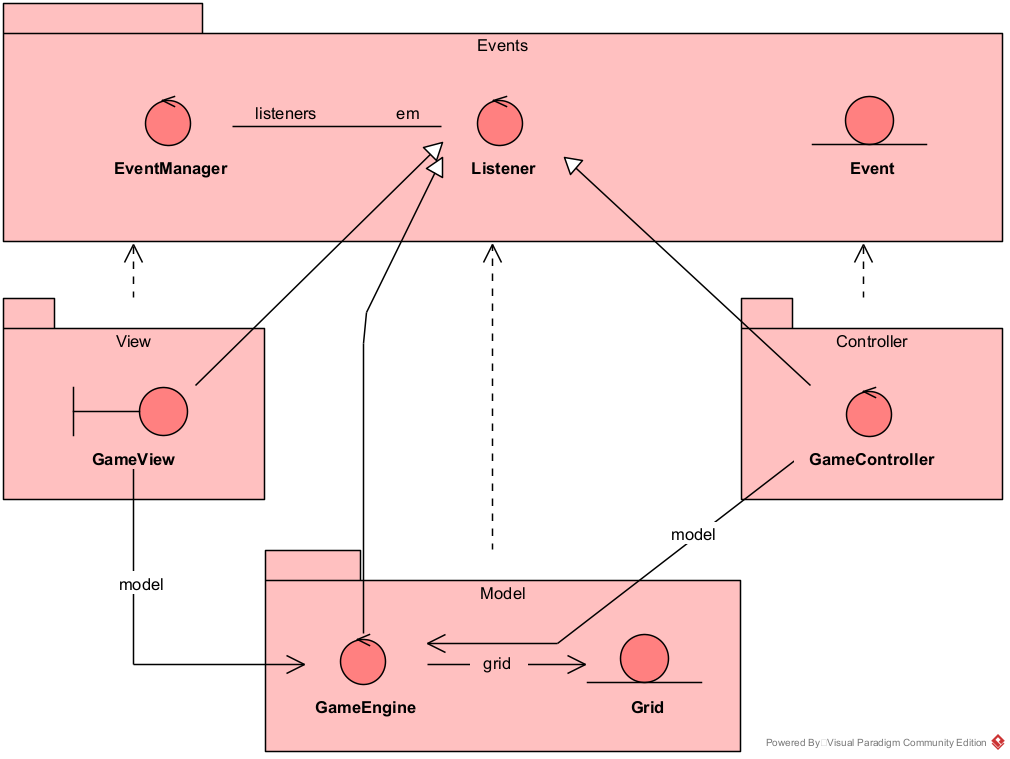
\includegraphics[scale=0.6]{img/mvc.png}
	\caption{Arquitectura del Sistema}
	\label{fig:arquitectura}
\end{figure}

A continuación se presenta una breve descripción de cada uno de los componentes que hacen parte de esta arquitectura.

\subsubsection{Model} \label{diseño:arquitectura:model}

El modelo guarda toda la lógica y estructura del estado del juego. Para lograr esto, se define un \textit{GameEngine} que se encarga de almacenar el estado del juego, así como modificarlo acorde a los eventos de modificación del modelo. Nótese que en el modelo se tiene la clase \textit{Grid}, la cual tiene toda la lógica de cómo funciona el juego. \par

\subsubsection{View} \label{diseño:arquitectura:view}

La vista se encarga de representar el estado actual del juego gráficamente en la pantalla. \textit{GameView} tiene toda la lógica asociada a pintar el modelo cada vez que se recibe un evento de actualización de pantalla. \par

\subsubsection{Controller} \label{diseño:arquitectura:controller}

El controlador se encarga de recibir todas las interacciones del usuario y llevarlas a modificar el modelo. \textit{GameController} tiene la lógica asociada a recibir los eventos de interacción del usuario y transformarlos en eventos de modificación del modelo. \par

\subsubsection{Events} \label{diseño:arquitectura:events}

Mediante los eventos se coordina toda la comunicación entre cada uno de los componentes. El \textit{EventManager} se encarga de manejar la cola de eventos y notificar a todos sus \textit{listeners asociados}. El \textit{Listener} es notificado cada vez que se genera un evento, y también tiene la posibilidad de colocar eventos en la cola. Nótese que \textit{GameEngine}, \textit{GameView} y \textit{GameController} heredan de este. \par

\subsection{Modelo de interacción del Sistema} \label{diseño:interaccion}

La interacción del Sistema y sus componentes está mediada por el manejador de eventos. En general, estos son los eventos de interacción importantes que analizar: \par

\begin{itemize}
    \item Inicialización, generado al ejecutar por primera vez el juego y el cual se encarga de inicializar todos los componentes del Sistema. 
    \item Tick, tick del reloj el cual se encarga de avisar a la Vista que debe actualizarse.
    \item Interacción del usuario, generado cuando el usuario interactúa con el Sistema y modifica el estado del modelo.
\end{itemize}

A continuación se presenta una breve representación de cada una de estas interacciones. \par

\subsubsection{Inicialización y Tick} \label{diseño:interaccion:inicializacion_tick}

En la figura \ref{fig:interaccion_init_tick} se presenta el modelo de interacción de inicialización y tick del reloj. La inicialización es dirigida por el modelo, el cual crea el evento de inicialización para los otros componentes. Después, entra en un ciclo hasta que el juego acabe que genera continuamente los ticks. La Vista utiliza estos para recuperar el estado del modelo y actualizarse. \par

\begin{figure}[ht!]
	\centering
	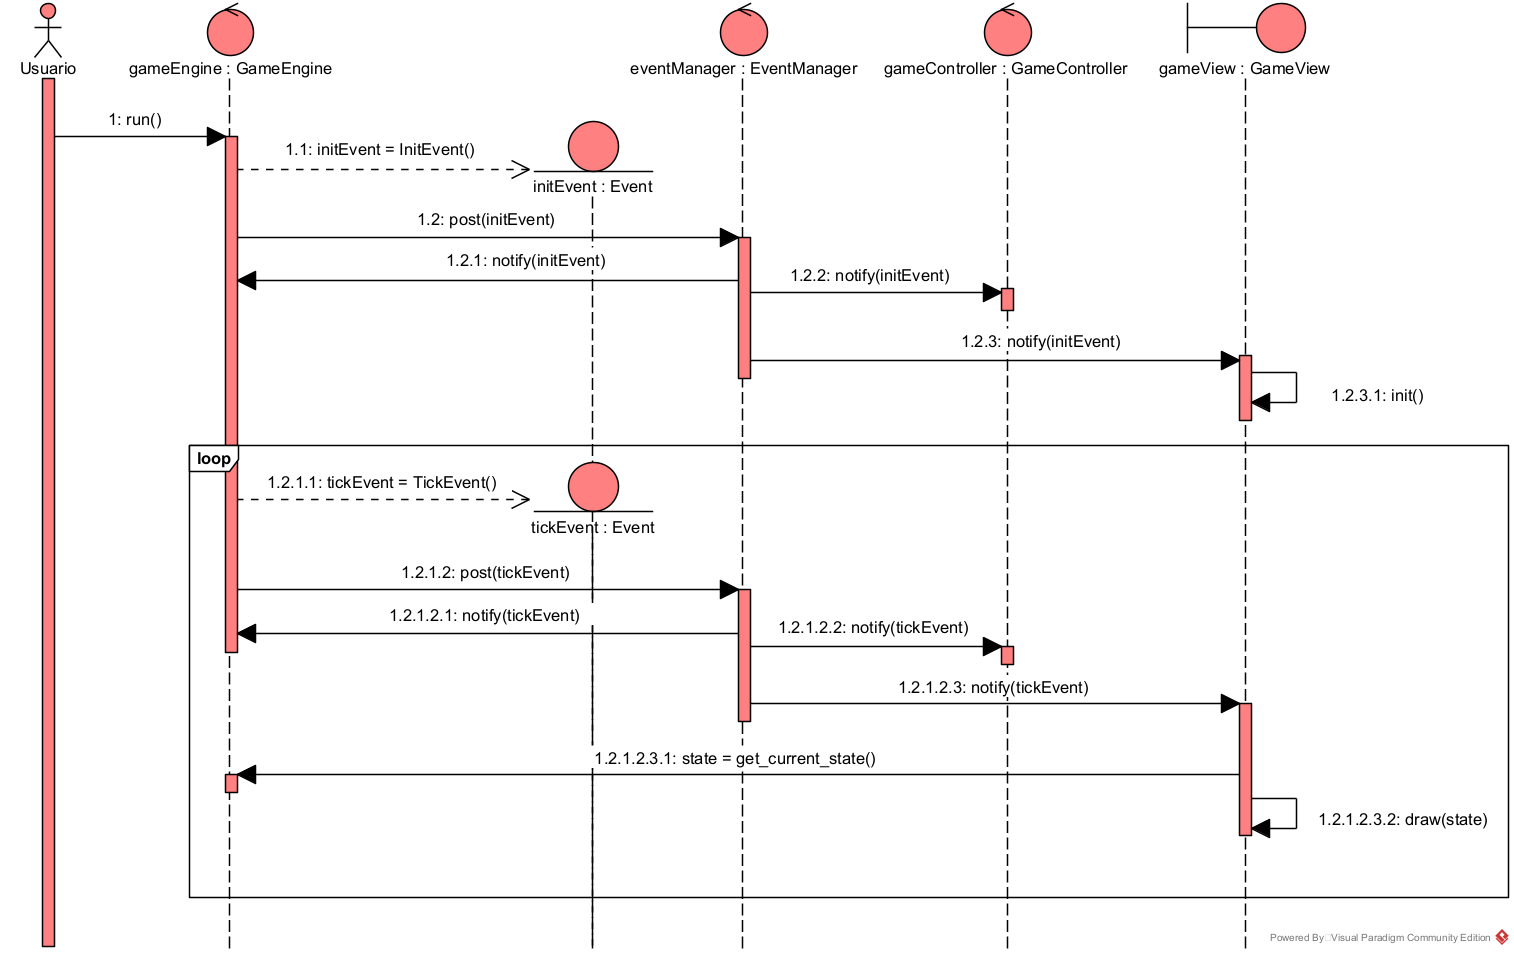
\includegraphics[scale=0.6]{img/sd_init_tick.png}
	\caption{Interacción de inicialización y tick del reloj}
	\label{fig:interaccion_init_tick}
\end{figure}

\subsubsection{Interacción del usuario} \label{diseño:interaccion:usuario}

En la figura \ref{fig:interaccion_usuario} se presenta el modelo de interacción del usuario. En general, el usuario interactúa con el controlador, el cual se encarga de traducir esta interacción en un evento de modificación del modelo (estado) del Sistema. \par

\begin{figure}[ht!]
	\centering
	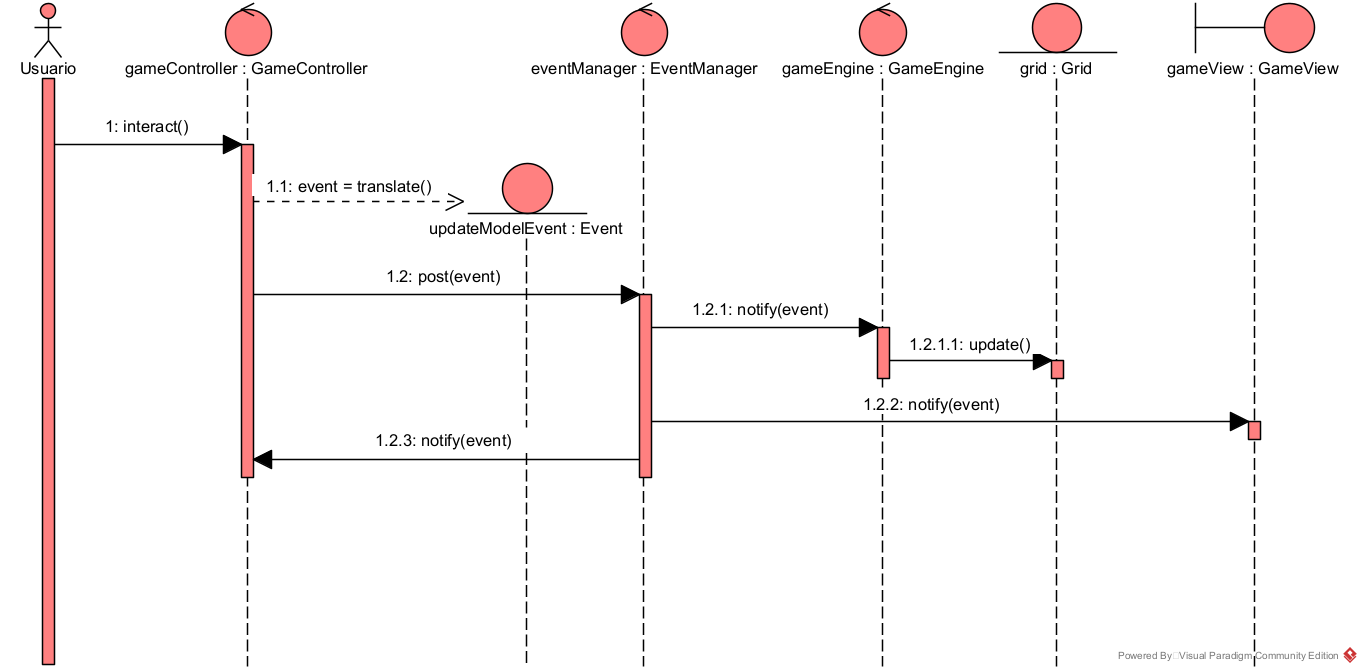
\includegraphics[scale=0.6]{img/sd_user_interaction.png}
	\caption{Interacción del usuario}
	\label{fig:interaccion_usuario}
\end{figure}

\subsection{Lógica del juego} \label{diseño:logica}

Como se mencionó en la sección \ref{diseño:arquitectura:model}, la lógica de cómo funciona el juego está mediada por el \textit{Grid}, el cual hace parte del estado del modelo. Como se vió en la sección \ref{diseño:interaccion:usuario}, la modificación del modelo (y por ende, del estado del juego) está dirigida por las interacciones del usuario. \par

\subsubsection{Representación del tablero} \label{diseño:logica:tablero}

Para empezar, se define el prototipo que modela el \textit{Grid}, presentado en la figura \ref{fig:prototipo_grid}. \par

\begin{figure}[ht!]
	\centering
	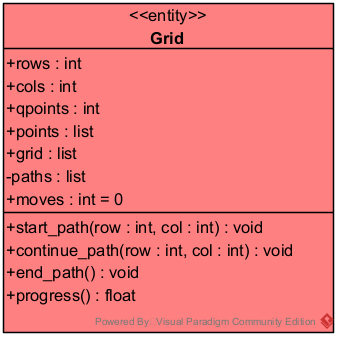
\includegraphics[scale=1]{img/cd_grid.png}
	\caption{Prototipo de \textit{Grid}}
	\label{fig:prototipo_grid}
\end{figure}

El tablero se modela a partir de una cantidad de filas (\textit{rows}), una cantidad de columnas (\textit{cols}), una cantidad de puntos (\textit{qpoints}) y el posicionamiento $(row, col)$ de cada par de puntos (\textit{points}). A partir de esta información, es posible construir el tablero (\textit{grid}): una matriz de $rows \times cols$. También se representan los caminos actuales (\textit{paths}): un arreglo de $(row, col)$ para cada punto disponible. \par

Cada celda del tablero es representada con un \textit{estado}, acorde a su color (un número entero) y su interacción (o no) con las demás celdas (dos números enteros de posicionamiento). Para entender el posicionamiento de una celda, véase la figura \ref{fig:posiciones_celda}. \par

\begin{figure}[ht!]
	\centering
	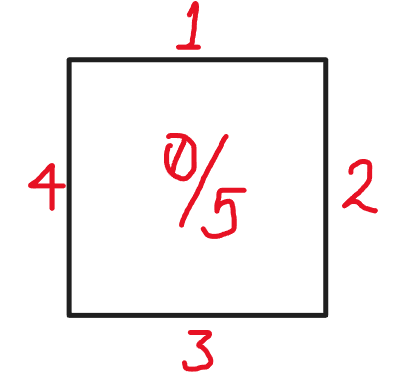
\includegraphics[scale=0.3]{img/cell_positions.png}
	\caption{Posiciones de una celda}
	\label{fig:posiciones_celda}
\end{figure}

Las posiciones cardinales norte, este, sur y oeste de una celda se representan con 1, 2, 3 y 4 respectivamente. Así mismo, el centro de celda puede ser representando con un 0 (inicio / fin) o un 5 (fin parcial). Estas posiciones se utilizan para representar como se posiciona la celda en el tablero. El posicionamiento entonces se refiere a de dónde viene el camino a la celda, y a dónde va el camino desde la celda. \par

Para entender mejor este concepto, supóngase que se tiene un tablero $3 \times 3$ con dos colores (rojo y azul) representados por los enteros 1 y 2 (con 0 como vacío) como el que se presenta en la figura \ref{fig:ejemplo_tablero_inicial}. Nótese en este que el posicionamiento de todas las celdas es $(0, 0)$, lo cual significa que no se han movido o no están conectadas por ningún camino. \par

\begin{figure}[ht!]
	\centering
	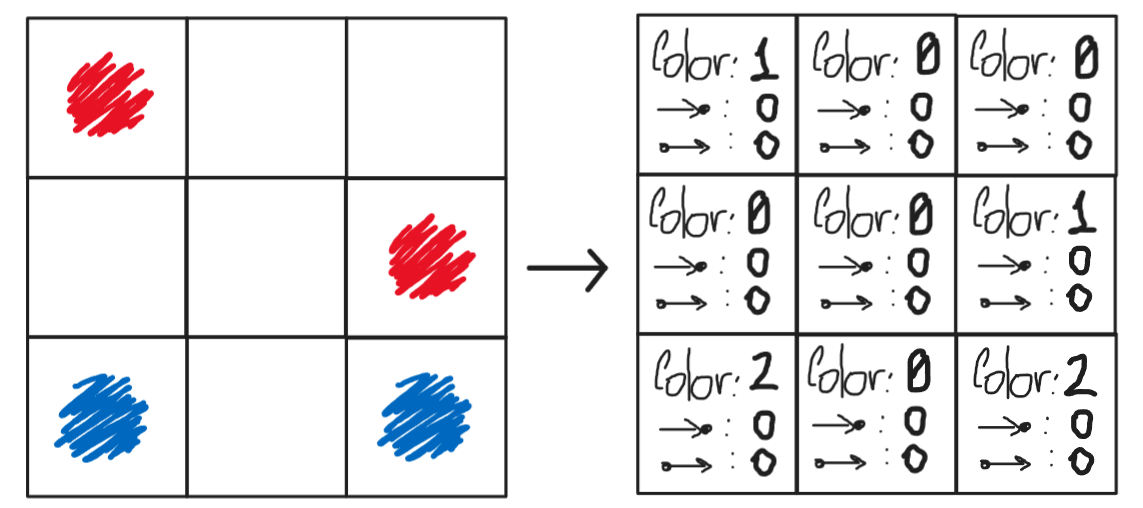
\includegraphics[scale=0.35]{img/example_grid_initial.png}
	\caption{Ejemplo de un tablero inicial}
	\label{fig:ejemplo_tablero_inicial}
\end{figure}

Tracemos un primer camino para el color rojo, desde su punto ubicado en la esquina superior izquierda como el que se presenta en la figura \ref{fig:ejemplo_tablero_mov1}. Nótese que el punto rojo ahora está representado como $(0,3)$, indicando que es un punto inicial que va hacia el sur. La última celda del camino rojo es $(3,5)$, indicando que un camino llega por el sur y se queda en el centro de la celda. \par

\begin{figure}[ht!]
	\centering
	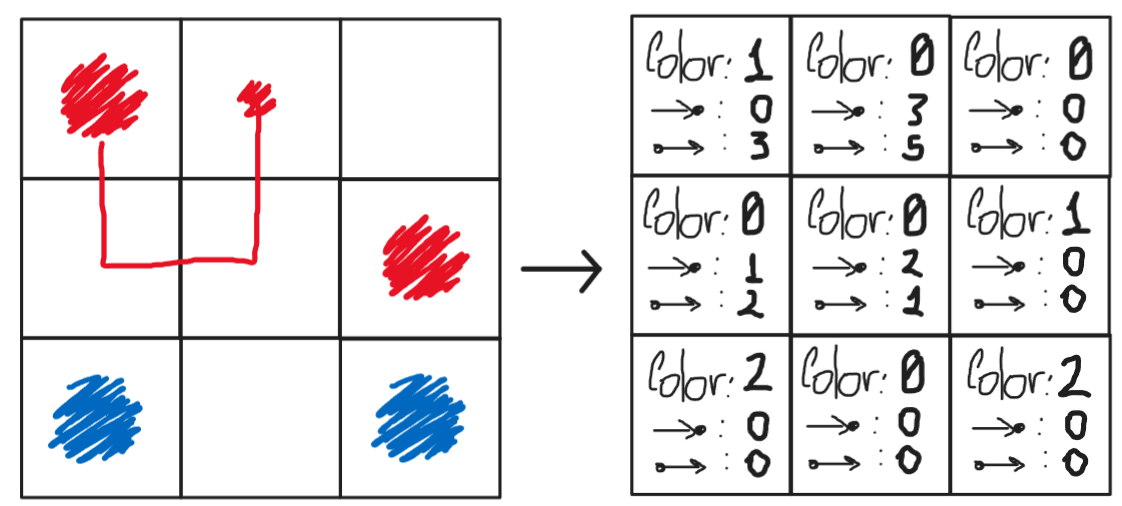
\includegraphics[scale=0.35]{img/example_grid_mov1.png}
	\caption{Ejemplo de un tablero primer movimiento}
	\label{fig:ejemplo_tablero_mov1}
\end{figure}

Un segundo camino para el color azul que conecta ambos puntos se presenta en la figura \ref{fig:ejemplo_tablero_mov2}. Nótese que el punto inicial es $(0,2)$ y el punto final es $(4,0)$, representando este último que un camino llega desde el oeste y termina en este punto. \par

\begin{figure}[ht!]
	\centering
	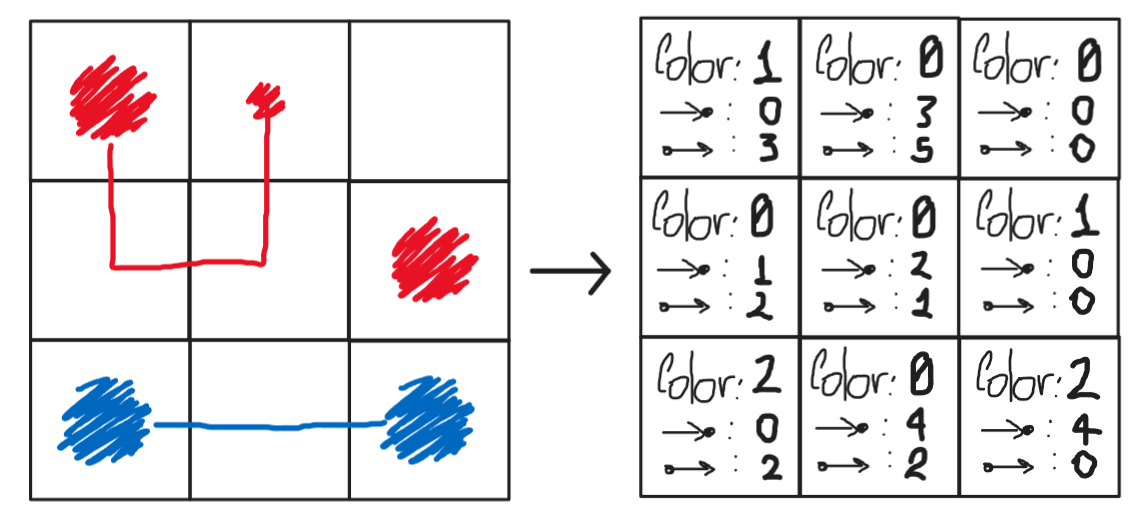
\includegraphics[scale=0.35]{img/example_grid_mov2.png}
	\caption{Ejemplo de un tablero segundo movimiento}
	\label{fig:ejemplo_tablero_mov2}
\end{figure}

\subsubsection{Interacción con el tablero} \label{diseño:logica:interaccion}

La interacción del usuario con el tablero se compone de 3 operaciones principales: \par

\begin{itemize}
    \item Iniciar un camino: el usuario hace un primer click sobre una celda que no está vacía. Esta interacción inicia un camino con el color de la celda sobre la que se para.
    \item Continuar un camino: el usuario continúa su click, moviendo el mouse por distintas celdas del tablero. Esta interacción continúa el camino del mismo color creado en el paso anterior.
    \item Terminar un camino: el usuario levanta el click. Esta interacción termina el camino que había sido iniciado.
\end{itemize}

\subsubsection{Iniciar un camino} \label{diseño:logica:iniciar}

En la figura \ref{fig:iniciar_camino} se presenta un flujograma con la lógica del juego al iniciar un camino. \par

\begin{figure}[ht!]
	\centering
	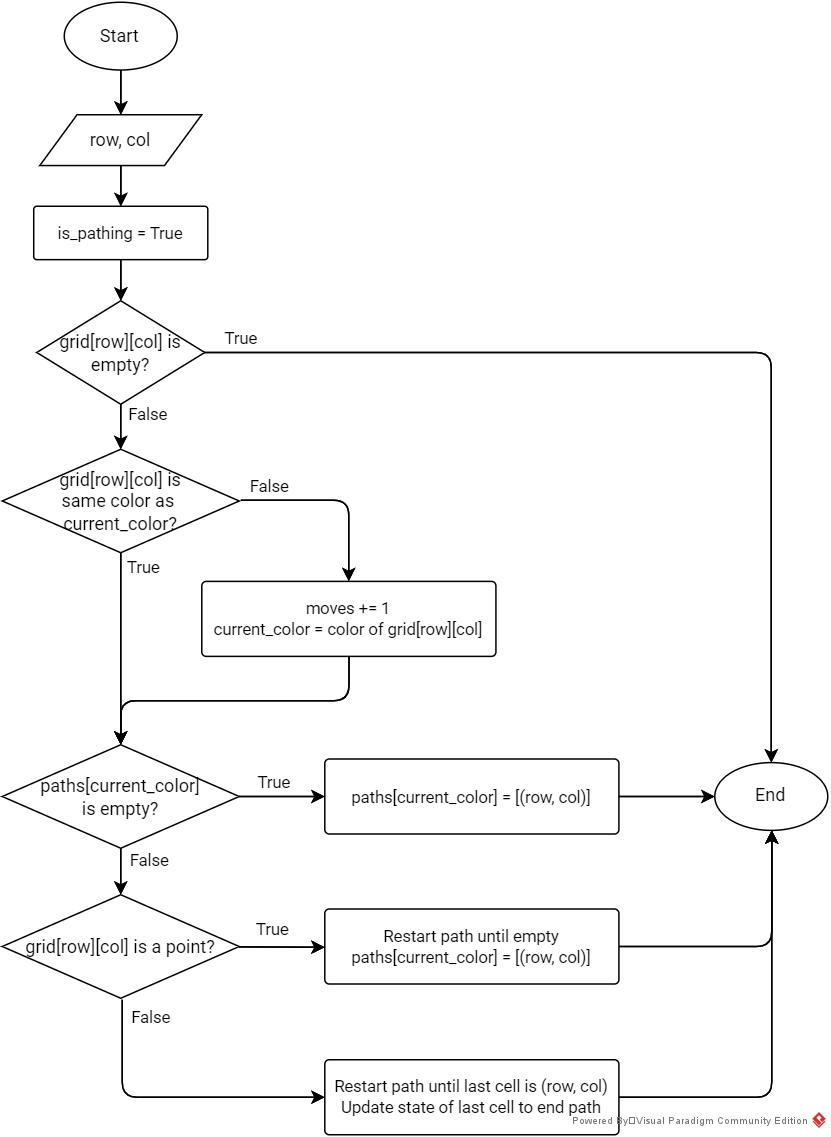
\includegraphics[scale=0.7]{img/fc_start_path.png}
	\caption{Flujograma de iniciar un camino}
	\label{fig:iniciar_camino}
\end{figure}

\subsubsection{Continuar un camino} \label{diseño:logica:continuar}

En la figura \ref{fig:continuar_camino} se presenta un flujograma con la lógica del juego al continuar un camino. \par

\begin{figure}[ht!]
	\centering
	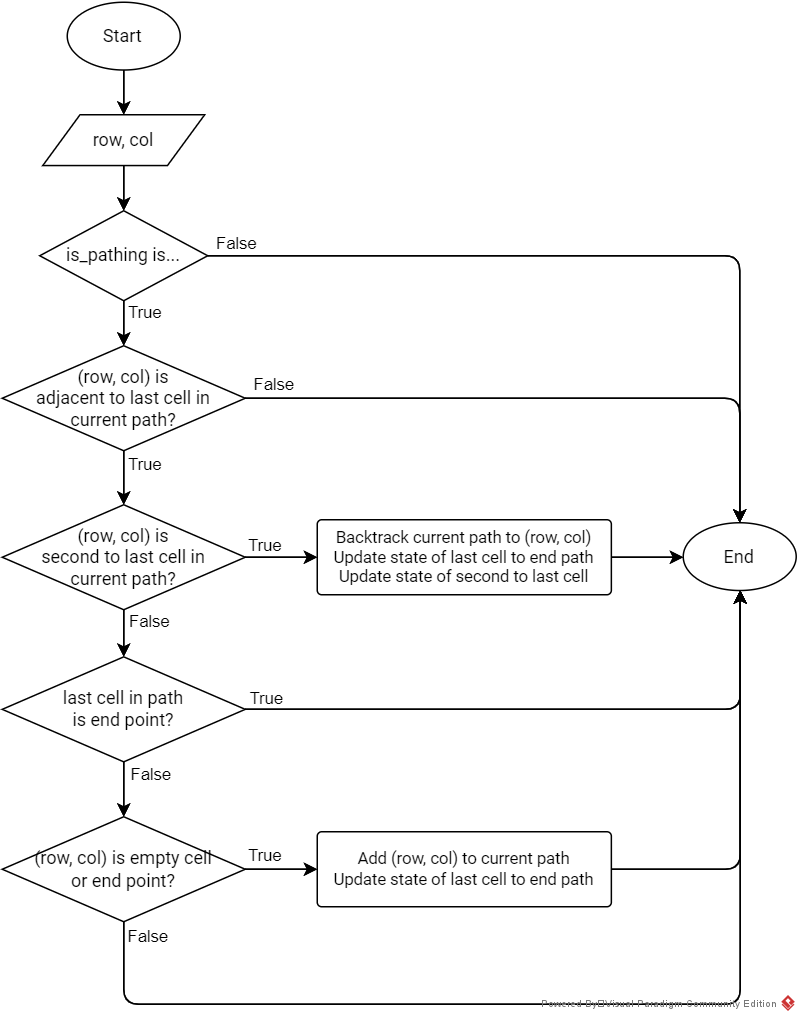
\includegraphics[scale=0.7]{img/fc_continue_path.png}
	\caption{Flujograma de continuar un camino}
	\label{fig:continuar_camino}
\end{figure}

\subsubsection{Terminar un camino} \label{diseño:logica:terminar}

En la figura \ref{fig:terminar_camino} se presenta un flujograma con la lógica del juego al terminar un camino. \par

\begin{figure}[ht!]
	\centering
	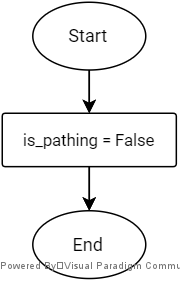
\includegraphics[scale=0.7]{img/fc_end_path.png}
	\caption{Flujograma de terminar un camino}
	\label{fig:terminar_camino}
\end{figure}



\section{Implementación} \label{implementacion}

El juego se desarrolla en Python v3.10. Para la implementación de las interfaces gráficas, se hace uso de la librería PyGame v2.1.2, la cual cuenta con múltiples módulos para facilitar la creación de videojuegos en Python. La implementación se hace acorde a la arquitectura definida en la sección \ref{diseño:arquitectura}, con el uso de la librería PyGame en la vista y el controlador. \par

\subsection{Vista previa del juego} \label{implementacion:vista_previa}

Una vista previa del juego se presenta en la figura \ref{fig:vista_previa}. \par

\begin{figure}[ht!]
	\centering
	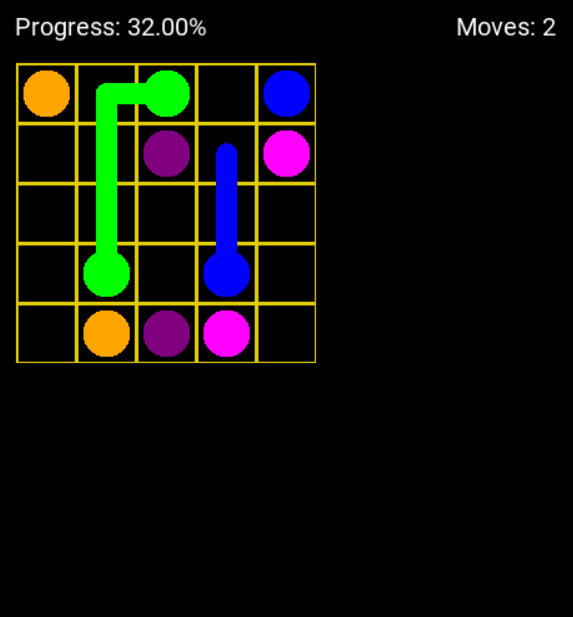
\includegraphics[scale=0.6]{img/game_preview.png}
	\caption{Vista previa del juego}
	\label{fig:vista_previa}
\end{figure}

\subsection{Funcionalidades del Sistema} \label{implementacion:funcionalidades}

Antes de empezar, el usuario tiene la posibilidad de: \par

\begin{itemize}
    \item Iniciar un juego con un tablero de niveles predeterminados
    \item Iniciar un juego con un tablero proporcionado en un archivo
    \item Iniciar un juego con un tablero creado al azar
\end{itemize}

Durante el juego, el usuario puede: \par

\begin{itemize}
    \item Crear caminos manteniendo presionado con el click derecho o izquierdo del mouse
    \item Reiniciar el tablero presionando la tecla R
    \item Ver en todo momento el progreso y cantidad de movimientos
\end{itemize}

\subsection{Restricciones del Sistema} \label{implementacion:restricciones}

Se definen las siguientes restricciones: \par

\begin{itemize}
    \item La cantidad mínima de puntos es 2 y la cantidad máxima es 16
    \item El tablero mínimo es de $2 \times 2$ y el máximo es de $15 \times 15$
\end{itemize}

\subsection{Configuración de los tableros} \label{implementacion:configuracion}

Como se mencionó en la sección \ref{implementacion:funcionalidades}, existen múltiples formas de iniciar un juego. Todas estas dependen de una configuración del tablero, la cual se representa como un diccionario en Python que contiene los mismos datos para representar un tablero (ver sección \ref{diseño:logica:tablero}). Por ejemplo, el mismo tablero inicial de la figura \ref{fig:ejemplo_tablero_inicial} es representado por la siguiente configuración: \par

\begin{verbatim}
{
   "rows": 3,
   "cols": 3,
   "qpoints": 2,
   "points": [
        [
            [0, 0], [1, 2]
        ],
        [
            [2, 0], [2, 2]
        ]
   ]
}
\end{verbatim}

Así mismo, esta configuración puede venir de niveles predeterminados, de un archivo o ser creada al azar. \par

\subsubsection{Tableros de niveles predeterminados} \label{implementacion:configuracion:niveles}

El juego viene con unos niveles predeterminados definidos dentro de un archivo JSON. Estos niveles aseguran que es posible ganar y existe una única solución. Refiérase a la sección \ref{documentacion:ejecucion:niveles} para ver como ejecutarlos. \par

\subsubsection{Tableros por archivos} \label{implementacion:configuracion:archivos}

Es posible definir una configuración similar a la presentada anteriormente dentro de un archivo JSON para proceder a jugar dicho tablero. Sin embargo, no es posible asegurar que se puede ganar. Refiérase a la sección \ref{documentacion:ejecucion:archivos} para ver como ejecutarlos. \par

\subsubsection{Tableros al azar} \label{implementacion:configuracion:azar}

Es posible definir una cantidad arbitraria de filas, columnas y puntos para que el juego genere un tablero al azar y poder proceder a jugarlo. Sin embargo, no es posible asegurar que se puede ganar. Refiérase a la sección \ref{documentacion:ejecucion:azar} para ver como ejecutarlos. \par

\newpage



\section{Análisis} \label{analisis}

\subsection{Formalización del Problema} \label{analisis:formalizacion}

Sean $n, m \in \mathbb{N}$ números naturales en el rango $[2, 9]$, sea $k \in \mathbb{N}$ un número natural en el rango $[2, 9]$ y sea $P = \langle ~ p_i \in \mathbb{N}^{2 \times 2} ~ | ~ i \in [1, k] \land j \in [1, 2] \land p_i^{[j]} = \langle x_i^{[j]}, y_i^{[j]} \rangle \land x_i \in [1,n] \land y_i \in [1,m] ~ \rangle$ como $k$ pares de puntos; es posible representar $T \in \mathbb{N}^{n \times m}$ una matriz compuesta por números naturales en el rango $0$ a $k$ tales que $T_{x_i^{[j]}, y_i^{[j]}} = i ~ \forall i \in [1, k] ~ \forall j \in [1, 2]$. Esto es, una matriz con las coordenadas dadas por el conjunto de puntos $P$ representadas como un $i$-índice del par de puntos o $0$ cuando no existe la coordenada en $P$. \par

El objetivo del problema es entonces \textit{conectar} todos los pares de puntos sobre el tablero $T$ de tal forma que $T_{x,y} \neq 0 ~ \forall x ~ \forall y$, no exista coordenada vacía en $T$. Así mismo, debe cumplirse que es posible ir desde $p_i^{[1]}$ hacia $p_i^{[2]}$ sobre $T$ para todo $i$. Defínase un vecino de $T_{x,y}$ como una coordenada adyacente a $(x,y)$ en cualquiera de las cuatro direcciones cardinales norte ($T_{x-1,y}$), sur ($T_{x+1,y}$), oeste ($T_{x,y-1}$) o este ($T_{x,y+1}$); siempre y cuando el vecino esté definido en el rango de búsqueda $\mathbb{N}^{n \times m}$. Una manera de determinar que este camino existe es que para todo $T_{x,y}=i$, este posee al menos dos vecinos con su mismo valor $i$ si $(x,y) \notin P$ o un vecino si $(x,y) \in P$. \par

\subsubsection{Definición del Problema ``Flow''} \label{analisis:formalizacion:definicion}

El problema ``Flow'' se define a partir de: \par

\begin{itemize}
    \item \textbf{Entradas:}
    \begin{itemize}
        \item $n \in \mathbb{N} ~ | ~ n \in [2,9]$, una cantidad de filas
        \item $m \in \mathbb{N} ~ | ~ m \in [2,9]$, una cantidad de columnas
        \item $k \in \mathbb{N} ~ | ~ k \in [2,9]$, una cantidad de pares de puntos
        \item $P = \langle ~ p_i \in \mathbb{N}^{2 \times 2} ~ | ~ i \in [1, k] \land j \in [1, 2] \land p_i^{[j]} = \langle x_i^{[j]}, y_i^{[j]} \rangle \land x_i \in [1,n] \land y_i \in [1,m] ~ \rangle$, una secuencia de pares de puntos
    \end{itemize}
    \item \textbf{Salidas:}
    \begin{itemize}
        \item $T \in \mathbb{N}^{n \times m} ~ | ~ T_{x,y} \in [1, k] ~ \forall x,y \land T_{x,y}$ posee al menos 2 vecinos si $(x,y) \notin P \lor T_{x,y}$ posee 1 vecino si $(x,y) \in P$.
    \end{itemize}
\end{itemize}

\subsubsection{Análisis del problema} \label{analisis:formalizacion:analisis}

Este problema se conoce en la literatura como un rompecabezas tipo \textit{Numberlink}, y se ha comprobado que es un problema de tipo decisión y de clase NP-completo. El algoritmo que lo soluciona ``perfectamente'' es permutativo y dadas las definiciones presentadas en la sección \ref{analisis:formalizacion:definicion}, esta solución tardaría un tiempo demasiado grande (complejidad temporal superpolinomial) en encontrar la solución. Es por esto que se propone abordar el problema mediante un algoritmo de aproximación. \par

\subsection{Algoritmo de Solución} \label{analisis:algoritmo}

\subsubsection{Idea general de la solución} \label{analisis:algoritmo:idea}

La primera idea que surge de un problema de este tipo, es desarrollar una solución por fuerza bruta. Sin embargo, como se mencionó en la sección anterior, este algoritmo puede demorar mucho debido a las condiciones establecidas. Entonces se empieza a abordar un algoritmo de aproximación. \par

El primer paso que se tomó fue el definir un tablero inicial dadas las restricciones de entrada como el que se muestra en la figura \ref{fig:grid_algo1}. Este particularmente, ya que se considera un desafío trazar el camino de los puntos azules sin interrumpir el de los amarillos. \par

\begin{figure}[ht!]
    \centering
    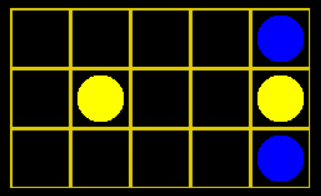
\includegraphics[scale=0.7]{img/grid_algo1.png}
    \vspace{-0.5em}
    \caption{Tablero inicial}
    \label{fig:grid_algo1}
\end{figure}

Deliberadamente, se procedió a tratar de simular un algoritmo que resuelva primero el camino azul y después el amarillo. Para lograr esto, se empezaron a definir unos costos asociados a las celdas de acuerdo a la distancia de Manhattan ($d(a,b) = |a_1 - b_1| + |a_2 - b_2|$) con el punto de partida y el punto de llegada, como se muestra en la figura \ref{fig:grid_algo2}. \par

\begin{figure}[ht!]
    \centering
    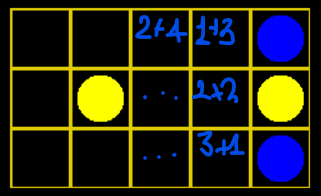
\includegraphics[scale=0.7]{img/grid_algo2.png}
    \vspace{-0.5em}
    \caption{Cálculo de costos inicial}
    \label{fig:grid_algo2}
\end{figure}

Sin embargo, se encontró un problema, y es que después de trazar el mejor camino azul y proceder a trazar el camino amarillo, no se encontraría ninguno, como se muestra en la figura \ref{fig:grid_algo3}. \par

\begin{figure}[ht!]
    \centering
    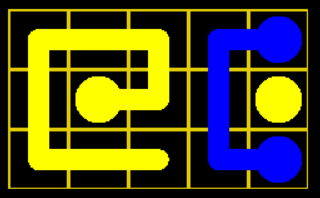
\includegraphics[scale=0.7]{img/grid_algo3.png}
    \vspace{-0.5em}
    \caption{Camino bloqueado}
    \label{fig:grid_algo3}
\end{figure}

Esta situación implicó la necesidad de implementar una especie de backtracking o el cálculo de mejores costos para tener mayores repercusiones sobre bloquear un camino de otro color. Se consideró entonces la posibilidad de acumular costos \textit{inversos}. Esto es, un camino para un color tiene el costo usual sumado con el costo inverso de los otros colores. Por ejemplo, el color amarillo tiene un costo de $1 + 2$ en la celda $(1,2)$, debido a que sus puntos tienen esa distancia a esa celda. El costo inverso sería el mayor costo (cantidad de celdas) menos el costo normal del color. De esta forma, se desincentiva bloquear los mejores caminos de otros colores, como se muestra en la figura \ref{fig:grid_algo4}. \par

\begin{figure}[ht!]
    \centering
    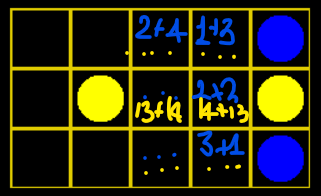
\includegraphics[scale=0.7]{img/grid_algo4.png}
    \vspace{-0.5em}
    \caption{Cálculo de costos inversos}
    \label{fig:grid_algo4}
\end{figure}

Sin embargo, rápido se desechó la anterior idea, debido a que una cantidad $k$ de puntos implica hacer $k * 2$ cálculos para saber el costo de una sola celda. Así mismo, situaciones como la que se presenta en la figura \ref{fig:grid_algo5} en donde existen varios colores cercanos, se desincentivaría el uso del camino correcto y se volvería a coger el camino más corto. \par

\begin{figure}[ht!]
    \centering
    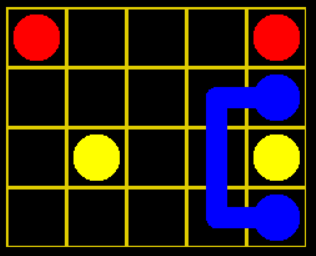
\includegraphics[scale=0.7]{img/grid_algo5.png}
    \vspace{-0.5em}
    \caption{Efecto adverso por más colores}
    \label{fig:grid_algo5}
\end{figure}

En este punto, se cayó en cuenta que la primera idea del algoritmo, de un doble costo asociado a la distancia origen y destino se parecen mucho al algoritmo de búsqueda A*, con la búsqueda del mejor camino entre 2 nodos. Es por esto que se toma esta idea y se decide utilizar el algoritmo A* para buscar el mejor camino entre cada par de puntos de cada color. Por cada par de puntos, se inicia en un punto y se empiezan a recorrer los vecinos siguiendo la lógica de prioridades y costos así:

\begin{itemize}
    \item $g(c) = g(c-1) + 1$, el costo de llegar a la siguiente celda como el costo de la celda padre más 1
    \item $h(c) = d(c,e)$, el costo heurístico de ir desde la siguiente celda hasta la celda fin como la distancia Manhattan entre estas
    \item $f(c) = g(c) + h(c)$
\end{itemize}

Al aplicar estas reglas y el algoritmo básico de A*, se encuentra que se está en una situación muy parecida a la inicial. Después de calcular el camino azul exactamente igual a como en la figura \ref{fig:grid_algo3} y determinar que es imposible trazar el camino amarillo, se necesita una forma de hacer backtracking sobre el camino azul para probar otro camino. A* no ofrece la posibilidad de determinar el N-avo mejor camino, por lo que siempre se va a recalcular el mismo camino azul. \par

Se propone entonces afectar los costos después de calcular un camino, para desincentivar recorrer el mismo camino la siguiente vez que se calcule A*. Para lograr esto, se implementa un efecto parecido a un mapa de calor, donde los caminos (y celdas) que se calculan continuamente con el algoritmo crecen en un costo que incentiva al algoritmo a buscar otros caminos. \par

La idea entonces es manejar una matriz de costos añadidos por cada color disponible, que se actualiza cada vez que se calcula un camino de un color. La matriz de costos añadidos crece en $n * m$ en cada celda visitada, con el fin de que sea más lucrativo recorrer todos los demás nodos que volver a pasar por uno ya visitado. Se puede entonces volver a representar $g(c)$ como: \par

\begin{itemize}
    \item $g(c) = g(c - 1) + 1 + a(c)$, el costo de llegar a una celda es el costo del camino existente más el costo añadido por repetir un camino sobre esa celda
    \item con $a(c) = a(c) + n * m$ cada vez que $c$ hace parte del camino solución
\end{itemize}

Finalmente, el algoritmo recorre todos los puntos disponibles calculando A* sobre el par de puntos. Cuando encuentra un camino, incrementa los pesos y pasa al siguiente punto. Si el siguiente punto queda en un punto muerto o se repite, se regresa al punto anterior para recalcular un nuevo camino. Los costos añadidos ayudan a que A* no calcule siempre el mismo camino, sino que recorra el espacio de búsqueda para encontrar caminos óptimos no explorados. \par

\subsubsection{Escritura del algoritmo} \label{analisis:algoritmo:escritura}

El algoritmo se basa principalmente en dos funcionalidades: encontrar un camino entre un par de puntos, y encontrar todos los caminos del tablero. Para encontrar todos los caminos, se utiliza la primera funcionalidad. \par

\newpage

\begin{algorithm}[ht!]
\caption{Calcular camino entre un par de puntos}
\begin{algorithmic}[1] 
\Procedure{SolvePoint}{$T, P, C, p$}
    \State $start \leftarrow P[p][0] \land end \leftarrow P[p][1]$
    \State $\textbf{let } q \textbf{ be a } \textsc{PriorityQueue}$
    \State $q.\Call{put}{0, start}$
    \State $\textbf{let } v \textbf{ be a } \textsc{Map}$
    \State $v[start] \leftarrow (0, \textsc{Null})$
    \State $ended \leftarrow 0$
    \While{$\textbf{not } q.\Call{Empty}{ } \land ended = 0$}
        \State $c \leftarrow queue.\Call{get}$
        \If{$c = end$}
            \State $ended \leftarrow 1$
        \EndIf
        \For{$n \textbf{ in } \Call{Neighbors}{c}$}
            \State $g \leftarrow v[c][0] + 1 + C[p][n]$
            \State $h \leftarrow \Call{Distance}{n, end}$
            \State $f \leftarrow g + h$
            \If{$n \textbf{ not in } v \lor v[n][0] > g$}
                \State $q.\Call{put}{f, n}$
                \State $v[n] \leftarrow (g, c)$
            \EndIf
        \EndFor
    \EndWhile
    \If{$end \textbf{ not in } v$}
        \State \Return $[~]$
    \EndIf
    \State $path \leftarrow [~]$
    \State $c \leftarrow end$
    \While{$c \textbf{ is not } \textsc{Null}$}
        \State $path \leftarrow c \cup path$
        \State $c \leftarrow v[c][1]$
        \State $C[p][c] \leftarrow C[p][c] + \textsc{AddedCost}$
    \EndWhile
    \State \Return $path$
\EndProcedure
\end{algorithmic}
\end{algorithm}

\newpage

\begin{algorithm}[ht!]
\caption{Solucionar tablero}
\begin{algorithmic}[1] 
\Procedure{Solve}{$T, P, C, k$}
    \State $p \leftarrow 1$
    \While{$1 \leq p \leq k$}
        \State $T.\Call{RemovePath}{p}$
        \State $path \leftarrow \Call{SolvePoint}{T, P, C, p}$
        \If{$path = [~]$}
            \State $p \leftarrow p - 1$
            \State \textbf{continue}
        \EndIf
        \State $T.\Call{AddPath}{path}$
        \If{$T.\Call{Progress}{ } = 1$}
            \State \Return $1$
        \EndIf
        \State $point \leftarrow point + 1$
    \EndWhile
    \State \Return $0$
\EndProcedure
\end{algorithmic}
\end{algorithm}

\subsection{Experimentación} \label{analisis:experimentacion}

Para la experimentación, se cuenta con 25 niveles importados de la aplicación \textit{Flow Free}, los cuáles garantizan una solución única. Son tableros desde $5 \times 5$ hasta $9 \times 9$, 5 niveles por tamaño.

\subsubsection{Prueba de completitud} \label{analisis:experimentacion:completitud}

El objetivo de esta prueba es determinar si el algoritmo implementado es capaz de resolver los 25 niveles disponibles. El protocolo de experimentación es:

\begin{enumerate}
    \item Se cargan los 25 niveles en el formato de configuración de tablero como se presenta en la sección \ref{implementacion:configuracion}.
    \item Cada nivel se corre el algoritmo con el comando \verb|python main.py -l LEVEL -s -d|. Más detalles en las secciones \ref{documentacion:ejecucion} y \ref{documentacion:solver}.
    \item Se determina si el algoritmo fue capaz de solucionar el tablero
\end{enumerate}

\subsubsection{Prueba de tiempo de ejecución} \label{analisis:experimentacion:tiempo}

El objetivo de esta prueba es determinar el tiempo que le toma al algoritmo solucionar distintas configuraciones de tableros. El protocolo de experimentación es:

\begin{enumerate}
    \item Se cargan los 25 niveles en el formato de configuración de tablero como se presenta en la sección \ref{implementacion:configuracion}.
    \item Se seleccionan los siguientes niveles que el algoritmo puede solucionar:
    \begin{itemize}
        \item Nivel 5: tablero $5 \times 5$ con $4$ pares de puntos
        \item Nivel 10: tablero $6 \times 6$ con $4$ pares de puntos
        \item Nivel 15: tablero $7 \times 7$ con $6$ pares de puntos
        \item Nivel 18: tablero $8 \times 8$ con $6$ pares de puntos
        \item Nivel 25: tablero $9 \times 9$ con $8$ pares de puntos
    \end{itemize}
    \item Se corre el algoritmo de solución 3 veces por cada nivel y se mide el tiempo de ejecución.
    \item Se promedian los tiempos de ejecución por cada nivel escogido.
\end{enumerate}

\subsection{Resultados} \label{analisis:resultados}

\subsubsection{Prueba de completitud} \label{analisis:resultados:completitud}

La prueba se sigue de acuerdo al protocolo establecido en la sección \ref{analisis:experimentacion:completitud}. Se determina que el algoritmo no es capaz de resolver los siguientes niveles / configuraciones:

\begin{itemize}
    \item Nivel 17: tablero $8 \times 8$ con $6$ pares de puntos
    \item Nivel 19: tablero $8 \times 8$ con $7$ pares de puntos
    \item Nivel 20: tablero $8 \times 8$ con $6$ pares de puntos
    \item Nivel 22: tablero $9 \times 9$ con $8$ pares de puntos
    \item Nivel 24: tablero $9 \times 9$ con $7$ pares de puntos
\end{itemize}

\subsubsection{Prueba de tiempo de ejecución} \label{analisis:resultados:tiempo}

La prueba se sigue de acuerdo al protocolo establecido en la sección \ref{analisis:experimentacion:tiempo}. Los resultados se presentan en la siguiente tabla:

\begin{table}[ht!]
\begin{tabular}{|l|r|}
\hline
\multicolumn{1}{|c|}{\textbf{Grid}} & \multicolumn{1}{c|}{\textbf{Average time (s)}} \\ \hline
$n=5, m=5, k=4$                       & $0.002658$                                       \\ \hline
$n=6, m=6, k=4$                       & $0.004479$                                       \\ \hline
$n=7, m=7, k=6$                       & $0.016763$                                       \\ \hline
$n=8, m=8, k=6$                       & $0.173835$                                       \\ \hline
$n=9, m=9, k=8$                       & $1.515127$                                       \\ \hline
\end{tabular}
\end{table}

Como se puede evidenciar, conforme el tamaño del tablero crece, el tiempo de ejecución crece a gran ritmo. Esto parece indicar que la complejidad del algoritmo obedece la de un polinomio de alto grado. \par

\newpage



\section{Documentación} \label{documentacion}

\subsection{Instalación} \label{documentacion:instalacion}

\subsubsection{Requisitos previos} \label{documentacion:instalacion:requisitos}

La máquina debe contar con la versión de Python 3.10 o superior.

\subsubsection{Windows} \label{documentacion:instalacion:windows}

Clonar el repositorio donde se aloja el código

\begin{verbatim}
> git clone https://github.com/amoralesc/flow.git
> cd flow
\end{verbatim}

Crear un entorno virtual para instalar las dependencias

\begin{verbatim}
> python -m venv venv
\end{verbatim}

(Opcional) Activar los permisos de ejecución de scripts

\begin{verbatim}
> Set-ExecutionPolicy -ExecutionPolicy RemoteSigned -Scope CurrentUser
\end{verbatim}

Activar el entorno virtual

\begin{verbatim}
> venv\Scripts\activate
\end{verbatim}

Instalar las dependencias

\begin{verbatim}
> pip install -r requirements.txt
\end{verbatim}

\subsubsection{Linux / Mac} \label{documentacion:instalacion:linux}

Clonar el repositorio donde se aloja el código

\begin{verbatim}
$ git clone https://github.com/amoralesc/flow.git
$ cd flow
\end{verbatim}

Crear un entorno virtual para instalar las dependencias

\begin{verbatim}
$ python -m venv venv
\end{verbatim}

Activar el entorno virtual

\begin{verbatim}
$ source venv/bin/activate
\end{verbatim}

Instalar las dependencias

\begin{verbatim}
$ pip install -r requirements.txt
\end{verbatim}

\subsection{Ejecución} \label{documentacion:ejecucion}

Para ver todas las opciones de ejecución posibles: \par

\begin{verbatim}
$ python main.py -h
\end{verbatim}

\subsubsection{Tableros de niveles predeterminados} \label{documentacion:ejecucion:niveles}

Para visualizar las configuraciones de tablero de los niveles disponibles: \par

\begin{verbatim}
$ cat data/levels.json
\end{verbatim}

Para ejecutar un tablero de un nivel predeterminado: \par

\begin{verbatim}
$ python main.py -l LEVEL
\end{verbatim}

donde \textsc{LEVEL} es un entero que representa la posición del nivel en el arreglo de niveles disponibles (indexado desde 1). \par

\subsubsection{Tableros por archivos} \label{documentacion:ejecucion:archivos}

Configurar previamente el tablero siguiendo los lineamientos de \ref{implementacion:configuracion} dentro de un archivo. Para ejecutar el tablero desde un archivo: \par

\begin{verbatim}
$ python main.py -f FILE
\end{verbatim}

donde \textsc{FILE} es la ruta hasta el archivo que contiene la configuración del tablero. \par

\subsubsection{Tableros al azar} \label{documentacion:ejecucion:azar}

Para ejecutar un tablero al azar: \par

\begin{verbatim}
$ python main.py -r ROWS COLS POINTS
\end{verbatim}

donde \textsc{ROWS}, \textsc{COLS} y \textsc{POINTS} son 3 enteros representando la cantidad de filas, columnas y puntos respectivamente. \par

\subsection{Solver} \label{documentacion:solver}

El programa cuenta con un solver que implementa el algoritmo descrito en la sección \ref{analisis:algoritmo}. Este solver se puede correr con cualquier de las opciones de ejecución presentadas anteriormente, agregando la bandera \verb|-s|. Por ejemplo, para correr el solver sobre el nivel 1: \par

\begin{verbatim}
$ python main.py -l 1 -s
\end{verbatim}

Así mismo, activando la bandera de debug \verb|-d|, es posible ver el paso a paso que el solver realiza para solucionar el tablero: \par

\begin{verbatim}
$ python main.py -l 1 -s -d
\end{verbatim}

El solver no garantiza encontrar una solución, así la configuración del tablero tenga una (o varias). \par

\subsection{Documentación del código}

El código se encuentra completamente documentado, y es posible referirse a este para entender las distintas partes de la implementación. \par

\end{document}
